\documentclass{article}
\usepackage[utf8]{inputenc}
\usepackage{authblk}
\usepackage{amsmath}
\usepackage{amssymb}
\usepackage{graphicx}
\usepackage{physics}
\usepackage{float}
\usepackage{bm}
\usepackage{caption}
\usepackage{subcaption}
\usepackage{dsfont}
\usepackage[parfill]{parskip}
\usepackage{blkarray}
\usepackage[dvipsnames]{xcolor}
\newcommand{\cj}{\mathcal{J}}
\newcommand{\cC}{\mathcal{C}}
\newcommand{\cE}{\mathcal{E}}
\newcommand{\cV}{\mathcal{V}}
\newcommand{\cK}{\mathcal{K}}
\newcommand{\Tau}{\mathcal{T}}

\newcommand{\matindex}[1]{\mbox{\scriptsize#1}}% Matrix index
\usepackage{geometry}
 \geometry{
 a4paper,
 left=25mm,
 right = 25 mm,
 top = 15mm,
 }

\title{QPC Project Status to 09.01.2025}
\author{Santiago Salazar Jaramillo}
\date{}

\begin{document}
\maketitle

\section{Summary}

The project aims is to develop a microscopic description of a QPC measuring a double dot system, including spin degrees of freedom. The QPC is represented as a tight-binding chain with a single gaussian wave-packet, which is coupled to the double dot (DD) only at a given site. It is expected that such a model will allow us to characterize the backaction on the DD beyond the results found in the literature, for example, by calculating entropy measures and including spin degrees of freedom. We are considering complementary numerical and analytical approaches. 

Regarding the analytics. For the decoupled case we have obtained the exact L-site QPC wavefunction and the frequency of the Rabi oscillations in the DD. The later is useful in gauging the back-action on the system. In addition, we have calculated the transmission probability of the QPC wave-packet in the decoupled case using scattering theory. This calculation has two key assumptions: First, the QPC particle is assumed to have a well defined trajectory (semiclassical limit) which is achieved by localizing it in $k$-space. Second, the DD hoping is assumed to be sufficiently small, so it can be approximated as a constant potential. Finally, we diagonalized the Hamiltonian block containing the DD and QPC bond sites. However, it was not clear how to incorporate this result (Landau-Büticker?).

Regarding numerics. We have a working Qutip code that uses exact diagonalization to solve the QPCxDD. The code has been shown to solve the decoupled case accurately (see \ref{sec:benchmark}) and to reproduce expected behaviors in the coupled case. In addition, an exploratory set of simulations has been conducted, in order to better understand how the different parameters influence the QPCxDD system. The main takeaways from the results shown in section \ref{sec:results} are :

\begin{itemize}
    \item We can measure how much the QPC affects the DD by the deviation from the decoupled case Rabi oscillations (Figure \ref{fig:effect_of_omega}). 
    \item  At larger DD hopping, the effect of the QPC is not noticeable (Figure \ref{fig:effect_of_omega}). 
    \item  The deviation from Rabi only appears after the particle has crossed the bond (Figure \ref{fig:effect_of_omega}).
    \item  The average momentum $k_{0}$ and bandwidth $\Delta x$ are the two variables that most affect hitting time (time it takes the QPC particle to reach the end of the chain) and time spent at bond (Figure \ref{fig:time_at_bond}).  
    \item  The estimation of the hitting time (explained below) is quite accurate for wavepackets with well defined trajectories (Figure \ref{fig:trajectories}).
    \item  There may be something wrong with the way we are incorporating the potential in the scattering calculation for the transmission coefficient (Figure \ref{fig:scattering}).
\end{itemize}

The following are the next tasks:
\begin{itemize}
    \item Calculate entanglement between double dot and QPC. How does it grow with time? How is it affected by the time spent at the bond?
    \item Go back to the literature and reproduce their results. 
    \item Develop a code that scales better with system size.
    \item Where are we applying the measurement postulate and why?
\end{itemize}


\section{Benchmark Example}\label{sec:benchmark}

Here we provide an example that shows the accuracy of the exact diagonalization algorithm in the decoupled case. Figure \ref{fig:benchmark} compares the numerical result with the exact one. The agreement between both is remarkable both in the QPC and the double dot. 

\begin{figure*}[t!]
    \centering
    \begin{subfigure}[t]{0.5\textwidth}
        \centering
        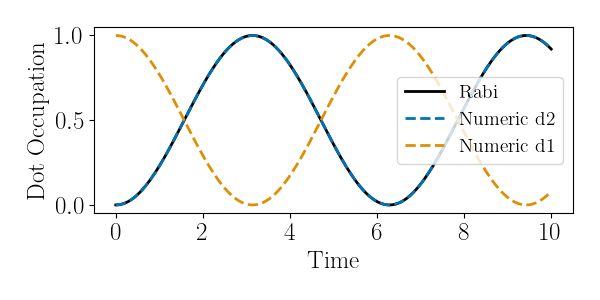
\includegraphics[width=\linewidth]{figures/decoupled_rabi_analytic_comp.png}
        \caption{}
    \end{subfigure}%
    \\
    \begin{subfigure}[t]{0.9\textwidth}
        \centering
        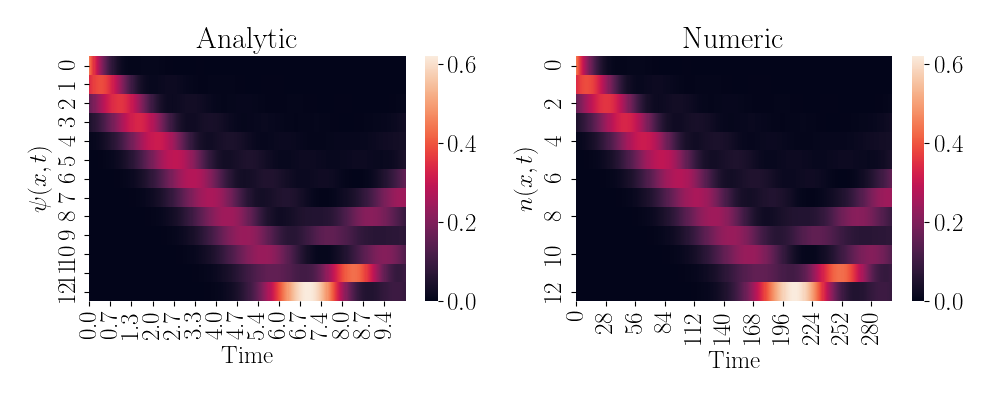
\includegraphics[width=\linewidth]{figures/decoupled_trajectories_analytic_comp.png}
        \caption{}
    \end{subfigure}\caption{Comparison between the numerical results and the exact solution for the decoupled case. (a) Rabi oscillations in the double dot, the solid line is exact. (b) Trajectories of the QPC wave-packet. The Analytical result shows the wavefunction and the numerical one the local densities $n(x,t)$.}\label{fig:benchmark}
\end{figure*}

This performance is consistent across different parameter regimes. 

\section{Data from Simulations}\label{sec:results}

The following are examples illustrating the observations mentioned above regarding the coupled case. 

Figure \ref{fig:effect_of_omega} shows two examples illustrating the effect that the QPC-DD coupling $\Omega$ has on the system. The plots show the deviation from the free Rabi oscillations on the DD as a result of the QPC backaction and how it is more pronounced in a low $t$ case. In addition, one can also see how the backaction kicks-in after the QPC electron hits the bond, as indicated by the dashed lines. 

\begin{figure*}[t!]
    \centering
    \begin{subfigure}[t]{0.5\textwidth}
        \centering
        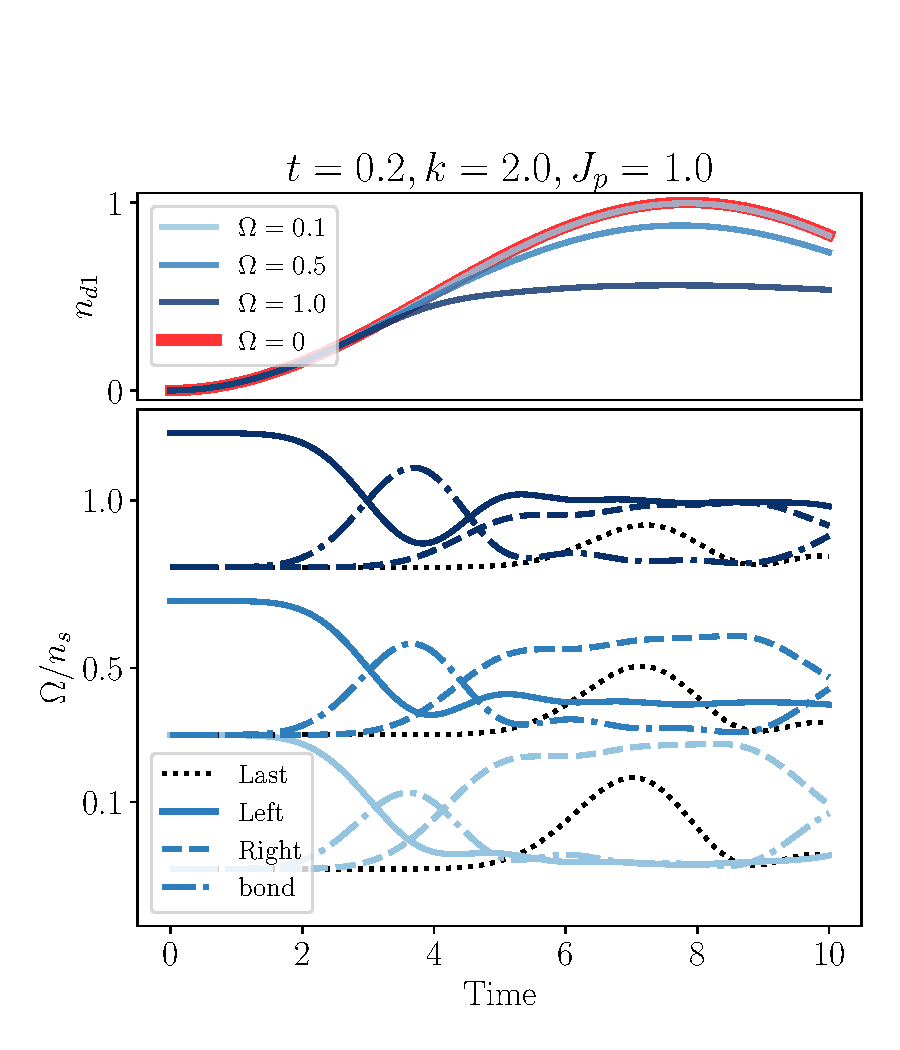
\includegraphics[width=\linewidth]{figures/density_sums_L=13.00_tdot=0.20_K=2.0_Jp=1.0_dd_second.pdf}
        \caption{}
    \end{subfigure}%
    \begin{subfigure}[t]{0.5\textwidth}
        \centering
        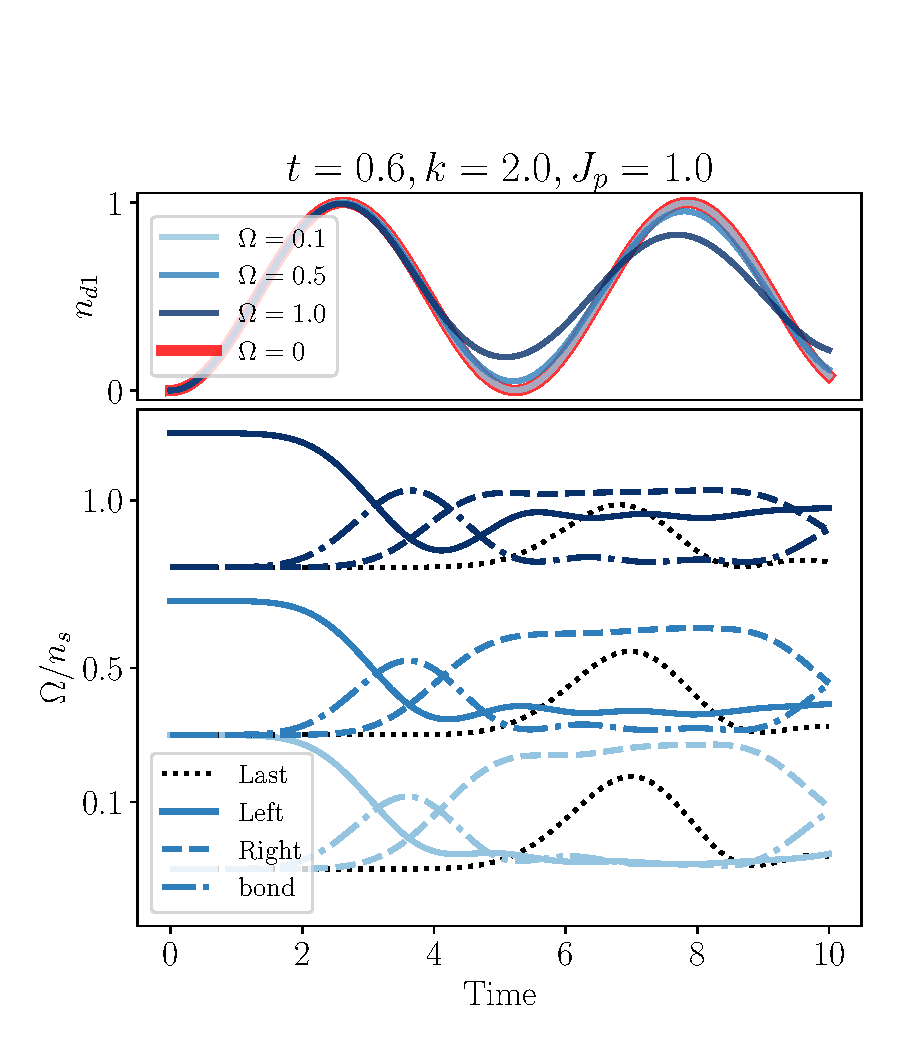
\includegraphics[width=\linewidth]{figures/density_sums_L=13.00_tdot=0.60_K=2.0_Jp=1.0_dd_second.pdf}
        \caption{}
\end{subfigure}\caption{Effect of the QPC-DD coupling $\Omega$ for two different values of the DD hopping $t$ in the semiclassical regime with $k_0=\Delta x =2.0$. Both cases have bond hopping $J_p =1$. The upper plot shows the oscillations in the double dot, while the ones at the bottom show the sums of the densities to the left and rifht of the bond (solid lines), at the bond (dashed line) and at the las QPC site (dotted line).}\label{fig:effect_of_omega}
\end{figure*}

To measure the hitting time (time it takes the QPC particle to reach the end of the chain), we have two equations: First, one that assumes there is no coupling between the QPC and Dot
\begin{equation}\label{eq:tau_free}
    \tau_{free} = \frac{m L}{v_{g}}
\end{equation}
where $v_{g}=\frac{\partial E}{\partial k}\vert_{k=k_{0}}, \, E=-2J\cos(k)$. The second assumes that we can separate the chain in three parts, before the bond (site where the DD coupling is located), directly at the bond and after the bond, such that
\begin{equation}\label{eq:tau_couple}
    \tau_{couple} = \tau_{\text{0 to B}}+\tau_{\text{at B}} + \tau_{\text{B to L}},
\end{equation}
where $\tau_{\text{0 to B}}$ $\tau_{\text{ to L}}$ are the times from the origin to bond and bond to the end, calculated as in \eqref{eq:tau_free} and $\tau_{\text{at B}}$ is the time spent at bond, which is calculated as the Full-Width-at-Half-Maximum of the bond density (dashed lines in figure \ref{fig:effect_of_omega}).

Figure \ref{fig:time_at_bond} shows that the time spent at bond and hitting time are mostly dependent on the wave-packet average momentum $k_0$, which makes sense since it is related to the group velocity.

\begin{figure*}[t!]
    \centering
    \begin{subfigure}[t]{0.4\textwidth}
        \centering
        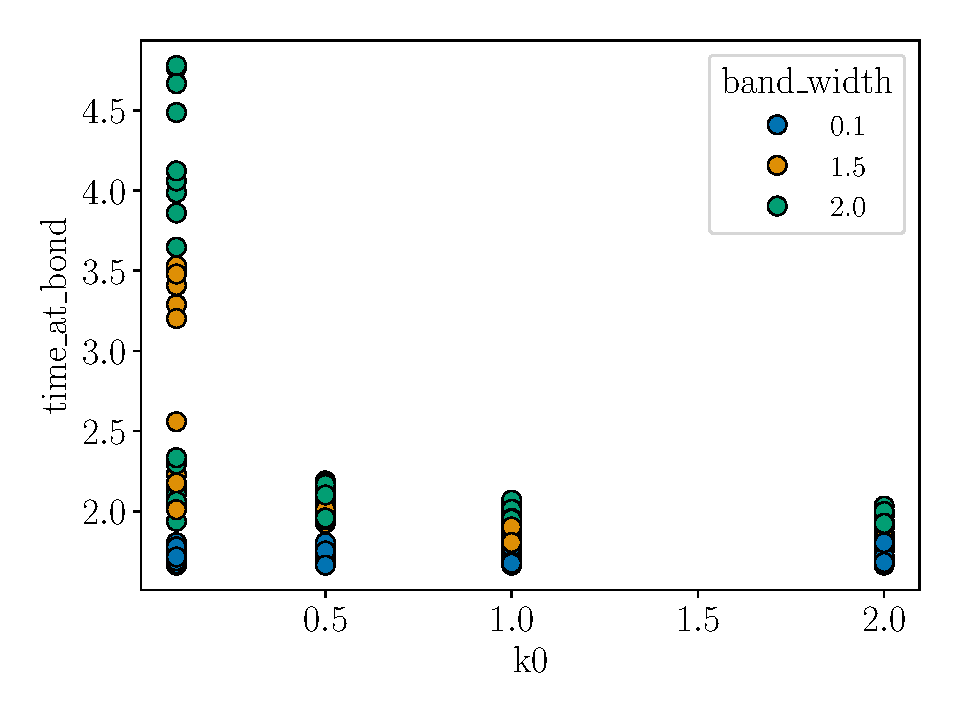
\includegraphics[width=\linewidth]{figures/time_at_bond_k0.pdf}
        \caption{}
    \end{subfigure}%
    
    \begin{subfigure}[t]{0.75\textwidth}
        \centering
        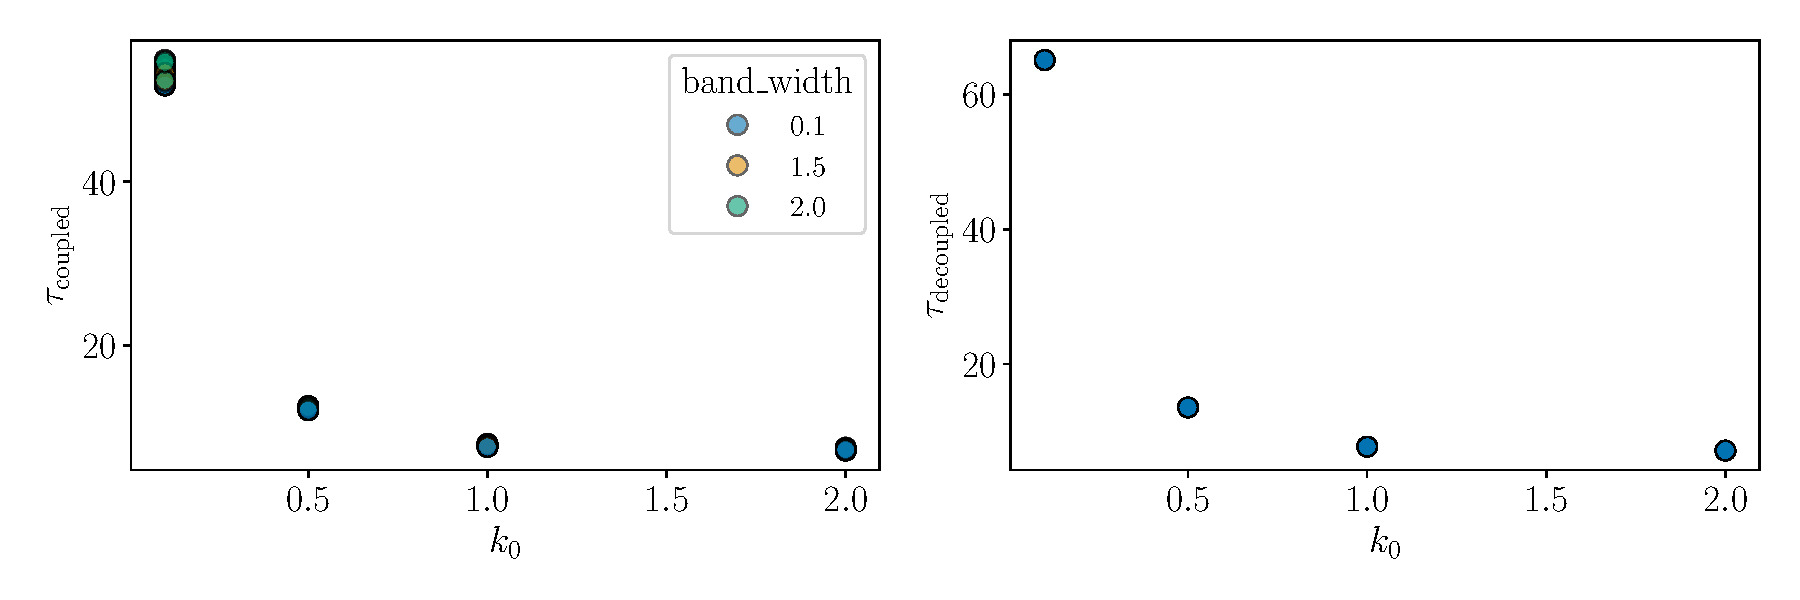
\includegraphics[width=\linewidth]{figures/hitting_time_k0.pdf}
        \caption{}
    \end{subfigure}\caption{Effect of the average wave-packet momentum $k_0$. (a) Time spent at bond (b) Time it takes the QPC to reach then end of the chain (Hitting time). The left plot for $\tau_{coupled}$ shows the hitting time estimation including the interaction at the bond (eq. \eqref{eq:tau_couple}) and the right one for $\tau_{free}$ is the time without the bond interaction (eq.\eqref{eq:tau_free})}\label{fig:time_at_bond}
\end{figure*}

Furthermore, we can compare how the estimated hitting times compare to the actual trajectories by plotting the local densities as done in figure \ref{fig:trajectories}. Here, it is clear that, when the QPC particle is in the semiclassical regime (left column) with well defined trajectories, the estimation of the hitting times is accurate. However, for a wave-packet strongly localized in space (right column), the estimation fails completely. 

\begin{figure*}[htb]
    \centering % <-- added
 \begin{subfigure}{0.4\textwidth}\hfill
 \caption{}
  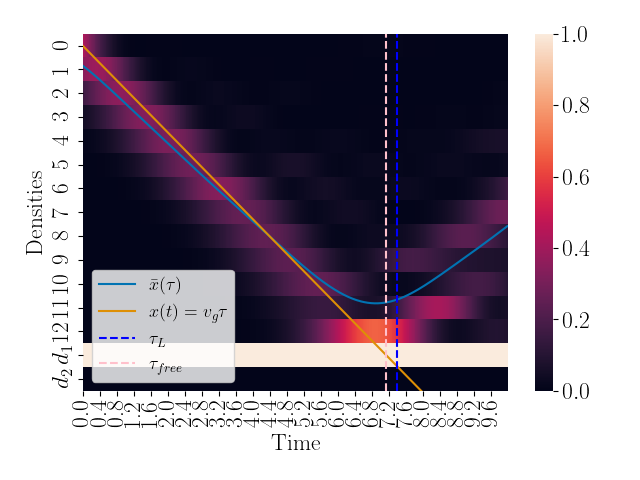
\includegraphics[width=\linewidth]{figures/traj_L=13_tdot=0.0_K=2.0_bw=2.0_Jp=1.0_om=0.1.png}
\end{subfigure} % <-- added
\begin{subfigure}{0.4\textwidth}\hfill
  \caption{}
  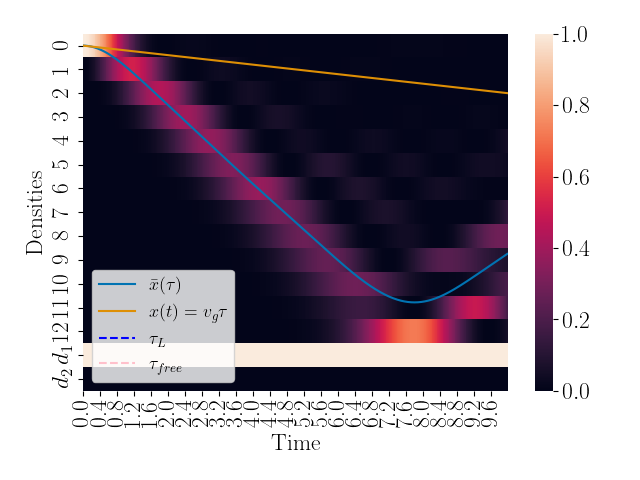
\includegraphics[width=\linewidth]{figures/traj_L=13_tdot=0.0_K=0.1_bw=0.1_Jp=1.0_om=0.1.png}
\end{subfigure}% <-- added

\centering % <-- added
 \begin{subfigure}{0.4\textwidth}\hfill
   \caption{}
  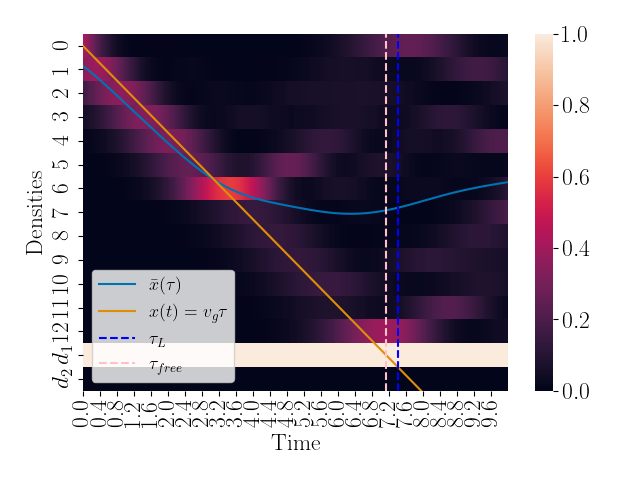
\includegraphics[width=\linewidth]{figures/traj_L=13_tdot=0.0_K=2.0_bw=2.0_Jp=1.0_om=0.5.png}
\end{subfigure} % <-- added
\begin{subfigure}{0.4\textwidth}\hfill
  \caption{}
  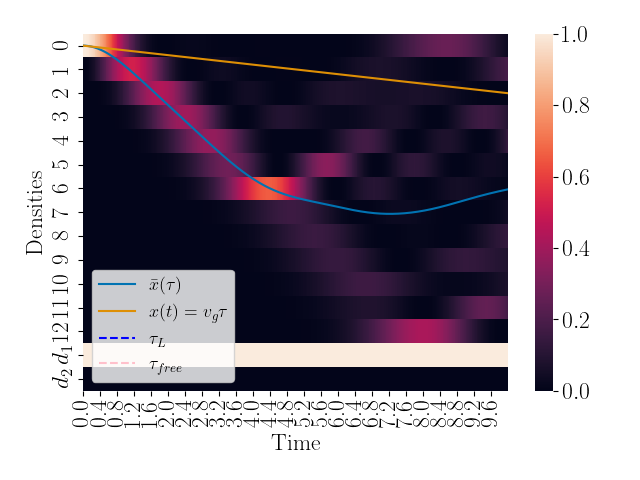
\includegraphics[width=\linewidth]{figures/traj_L=13_tdot=0.0_K=0.1_bw=0.1_Jp=1.0_om=0.5.png}
\end{subfigure}% <-- added

\centering % <-- added
 \begin{subfigure}{0.4\textwidth}\hfill
   \caption{}
  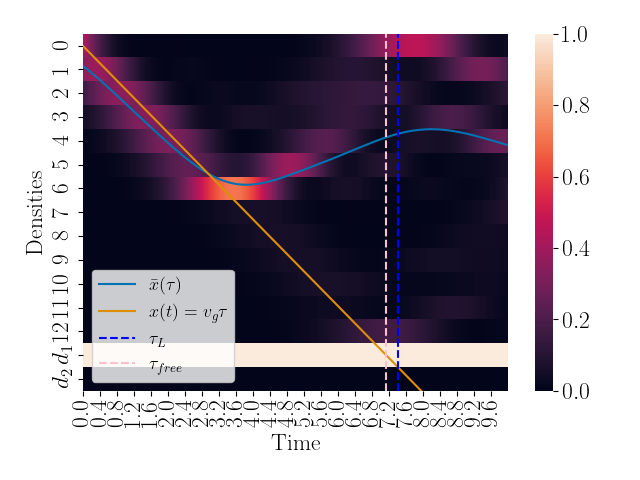
\includegraphics[width=\linewidth]{figures/traj_L=13_tdot=0.0_K=2.0_bw=2.0_Jp=1.0_om=0.7.png}
\end{subfigure} % <-- added
\begin{subfigure}{0.4\textwidth}\hfill
  \caption{}
  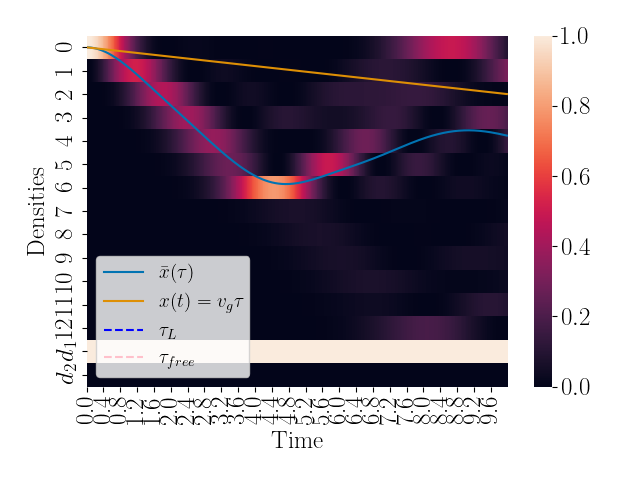
\includegraphics[width=\linewidth]{figures/traj_L=13_tdot=0.0_K=0.1_bw=0.1_Jp=1.0_om=0.7.png}
\end{subfigure}% <-- added
\caption{QPC trajectories for several examples. The columns with (a), (c), (d) shows cases in the semiclassical regime with $k_0 = \Delta x = 2.0$ at increasing coupling $\Omega = 0.1, \; 0.5, \; 0.7$ (top to bottom). Plots (b), (d), (f) show examples without well defined trajectories ($k_0 = \Delta  = 0.1$) for the same values of $\Omega$. The solid lines represent the average position from the numerics ($\title{x}(t)$) and free case expectation ($x(t)$). The dashed lines correspond to the two hitting time estimations.}\label{fig:trajectories}
\end{figure*}

This calculation can also be compared to expectations from scattering (assuming that the DD hopping is small enough) by calculating the transmission probabilities of the wave-packet. The total transmission probability is
\begin{equation}
    T_{tot} = \sum_k T(k) p(k),
\end{equation}
where $p(k)$ is a gaussian and 
\begin{equation}
    T(k) = \frac{1}{1+\left(\frac{m V_0}{\hbar^2 k}\right)^2}
\end{equation}
is the transmission probability for each momentum $k$. The potential is approximated from the bond interaction as $V_0 = J-2(\Omega + J_p)$ where $J$, $J_p$ are the QPC hopings. 

Figure \ref{fig:scattering} shows the results for the same cases as in figure \ref{fig:trajectories} by comparing the transmission probability with the sum of the densities to the right of the bond. Here, it is clear that there is a significant discrepancy between both quantities for weaker and stronger $\Omega$ but both agree at $\Omega \approx 0.5$. I believe this is due to the way we are calculating $V_0$.

\begin{figure*}[htb]
    \centering % <-- added
 \begin{subfigure}{0.4\textwidth}\hfill
 \caption{}
  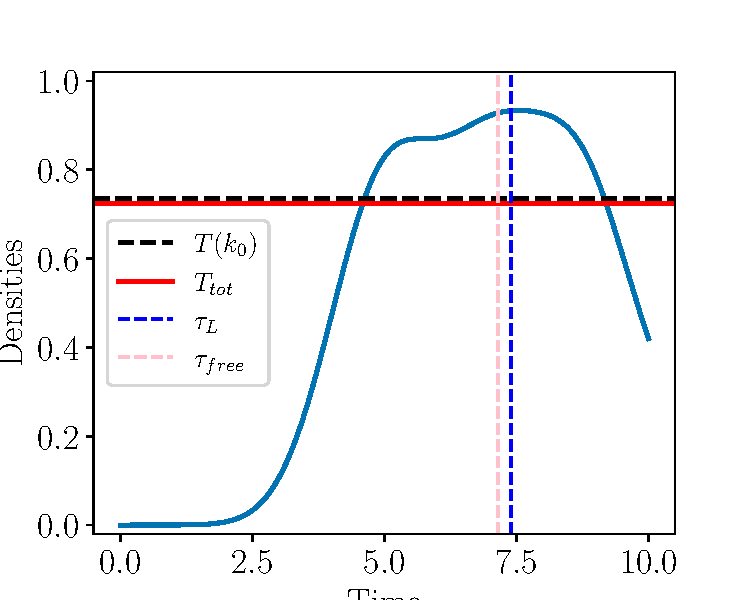
\includegraphics[width=\linewidth]{figures/scattering_L=13_tdot=0.0_K=2.0_bw=2.0_Jp=1.0_om=0.1.pdf}
\end{subfigure} % <-- added
\begin{subfigure}{0.4\textwidth}\hfill
  \caption{}
  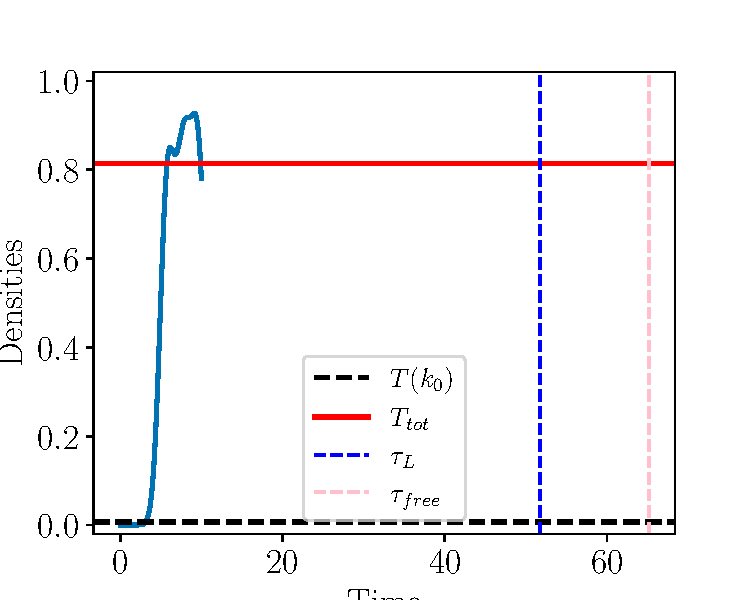
\includegraphics[width=\linewidth]{figures/scattering_L=13_tdot=0.0_K=0.1_bw=0.1_Jp=1.0_om=0.1.pdf}
\end{subfigure}% <-- added

\centering % <-- added
 \begin{subfigure}{0.4\textwidth}\hfill
   \caption{}
  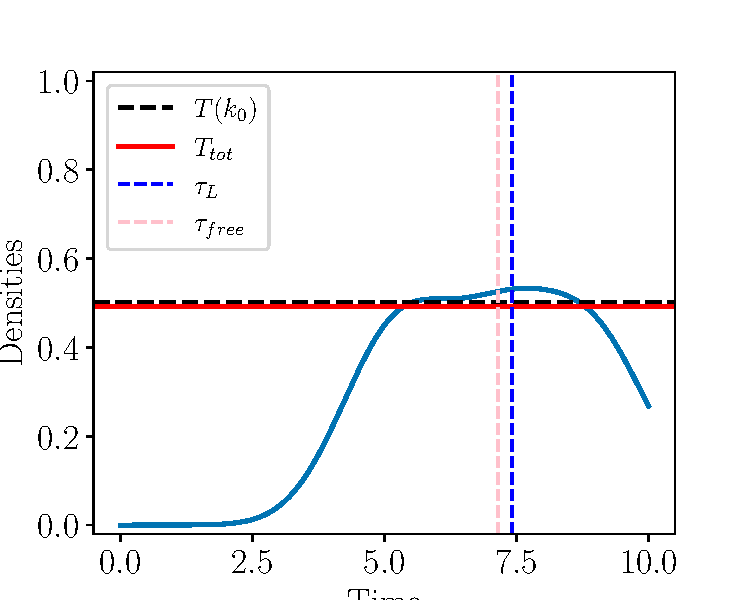
\includegraphics[width=\linewidth]{figures/scattering_L=13_tdot=0.0_K=2.0_bw=2.0_Jp=1.0_om=0.5.pdf}
\end{subfigure} % <-- added
\begin{subfigure}{0.4\textwidth}\hfill
  \caption{}
  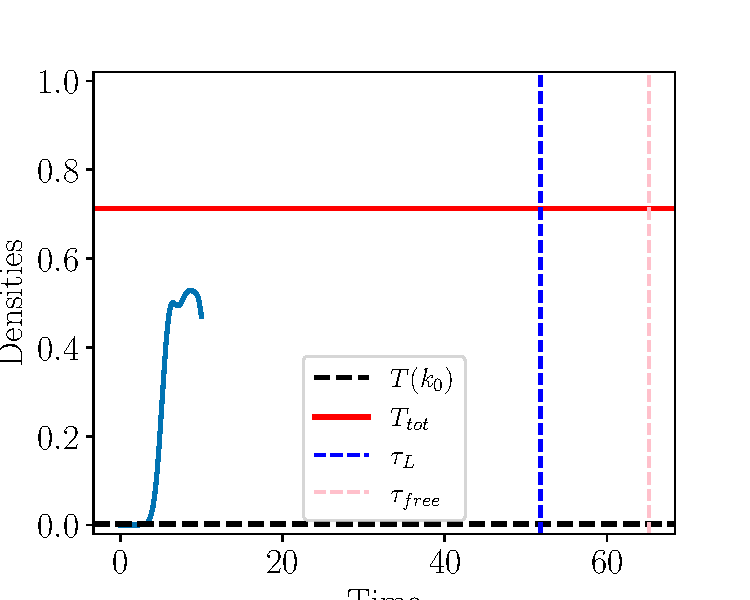
\includegraphics[width=\linewidth]{figures/scattering_L=13_tdot=0.0_K=0.1_bw=0.1_Jp=1.0_om=0.5.pdf}
\end{subfigure}% <-- added

\centering % <-- added
 \begin{subfigure}{0.4\textwidth}\hfill
   \caption{}
  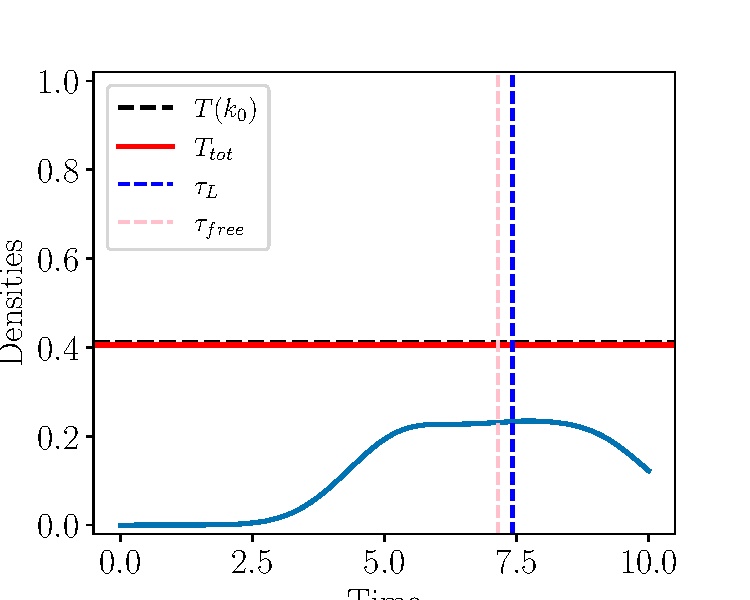
\includegraphics[width=\linewidth]{figures/scattering_L=13_tdot=0.0_K=2.0_bw=2.0_Jp=1.0_om=0.7.pdf}
\end{subfigure} % <-- added
\begin{subfigure}{0.4\textwidth}\hfill
  \caption{}
  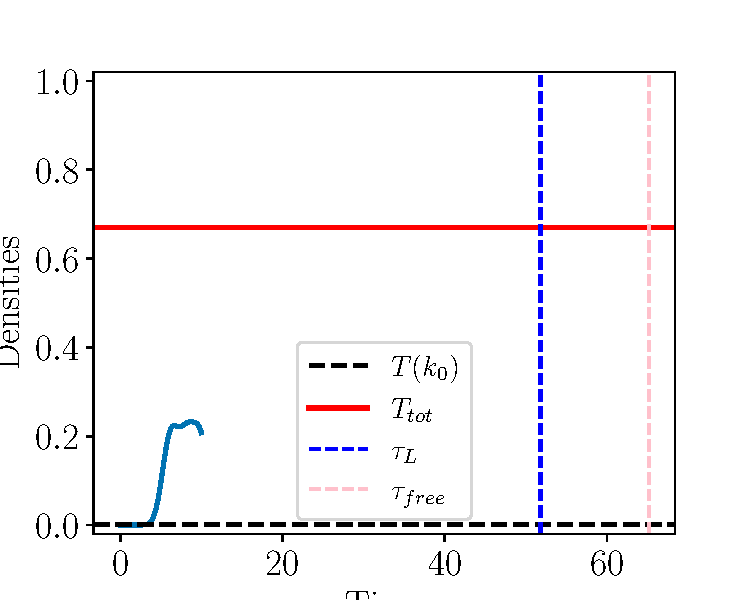
\includegraphics[width=\linewidth]{figures/scattering_L=13_tdot=0.0_K=0.1_bw=0.1_Jp=1.0_om=0.7.pdf}
\end{subfigure}% <-- added
\caption{Comparison between the sum of the densities to the left of the bond (solid blue line) to the scattering transmission probabilities (red line and dashed line). The vertical lines show the hitting times. The examples correspond to those shown in \ref{fig:trajectories}.}\label{fig:scattering}
\end{figure*}

\end{document}
